\documentclass[border=10pt]{standalone}
\usepackage{xcolor}
\usepackage{tikz}
\usetikzlibrary{arrows.meta}

\definecolor{BG}{HTML}{FAFAFA}
\definecolor{INK}{HTML}{1A1A2E}
\definecolor{SUB}{HTML}{555566}
\definecolor{COLD}{HTML}{4361EE}
\definecolor{PART}{HTML}{89B4F7}

\begin{document}
\pagecolor{BG}
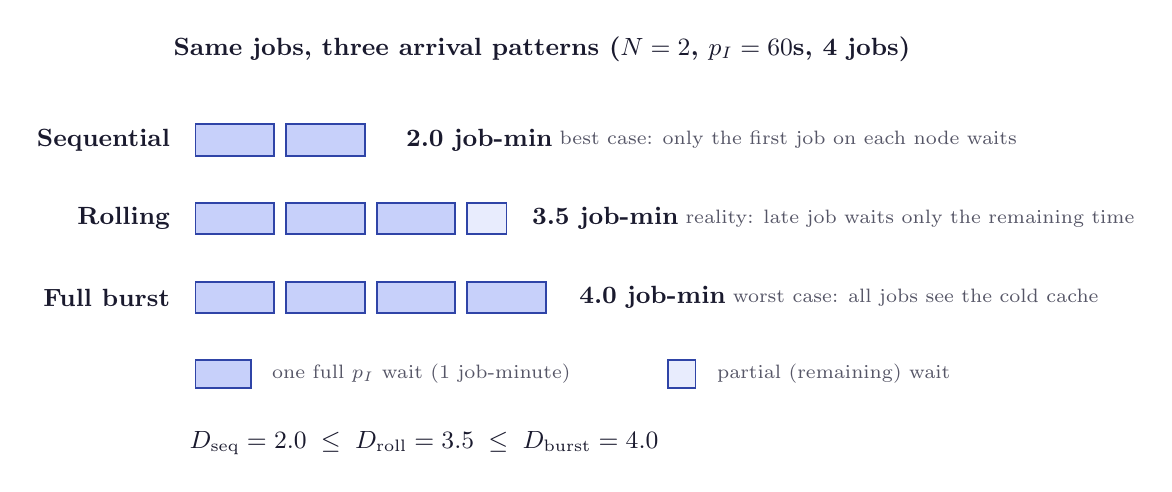
\begin{tikzpicture}[
  font=\sffamily,
  full/.style={fill=COLD!30, draw=COLD!70!black, line width=0.7pt},
  part/.style={fill=COLD!12, draw=COLD!70!black, line width=0.7pt},
  rowlabel/.style={font=\small\bfseries, text=INK, anchor=east},
  val/.style={font=\small\bfseries, text=INK, anchor=west},
  note/.style={font=\scriptsize, text=SUB},
  head/.style={font=\small\bfseries, text=INK},
]

\node[head] at (4.4, 3.75) {Same jobs, three arrival patterns (\(N=2\), \(p_I=60\)s, 4 jobs)};

% each full block = 1 job-minute (one full p_I wait)
% Sequential: 2.0
\node[rowlabel] at (-0.2, 2.6) {Sequential};
\foreach \i in {0,1} { \draw[full] (\i*1.15, 2.4) rectangle (\i*1.15+1.0, 2.8); }
\node[val] at (2.55, 2.6) {2.0 job-min};
\node[note, anchor=west] at (4.5, 2.6) {best case: only the first job on each node waits};

% Rolling: 3.5
\node[rowlabel] at (-0.2, 1.6) {Rolling};
\foreach \i in {0,1,2} { \draw[full] (\i*1.15, 1.4) rectangle (\i*1.15+1.0, 1.8); }
\draw[part] (3.45, 1.4) rectangle (3.45+0.5, 1.8);
\node[val] at (4.15, 1.6) {3.5 job-min};
\node[note, anchor=west] at (6.1, 1.6) {reality: late job waits only the remaining time};

% Burst: 4.0
\node[rowlabel] at (-0.2, 0.6) {Full burst};
\foreach \i in {0,1,2,3} { \draw[full] (\i*1.15, 0.4) rectangle (\i*1.15+1.0, 0.8); }
\node[val] at (4.75, 0.6) {4.0 job-min};
\node[note, anchor=west] at (6.7, 0.6) {worst case: all jobs see the cold cache};

% legend
\draw[full] (0, -0.55) rectangle (0.7, -0.2);
\node[note, anchor=west] at (0.85, -0.375) {one full \(p_I\) wait (1 job-minute)};
\draw[part] (6.0, -0.55) rectangle (6.35, -0.2);
\node[note, anchor=west] at (6.5, -0.375) {partial (remaining) wait};

\node[font=\small\bfseries, text=INK, anchor=west] at (-0.2, -1.25)
  {\(D_{\mathrm{seq}} = 2.0 \;\le\; D_{\mathrm{roll}} = 3.5 \;\le\; D_{\mathrm{burst}} = 4.0\)};

\end{tikzpicture}
\end{document}
